\documentclass[user_manual.tex]{subfiles}
\begin{document}
 
 \chapter{Software}
\section{ROS Introducción}
ROS es un \textit{middleware} de código abierto (open source) que provee la funcionalidad comúnmente necesaria en el 
desarrollo de software para robots moviles autonomos, como paso de mensajes y manejo de paquetes. La robot Justina 
utiliza ROS como plataforma de desarrollo.\\

ROS puede describirse en dos niveles conceptuales: el sistema de archivos y el grafo de
procesos.\\

El sistema de archivos. Se refiere al modo en que están organizados los recursos en
disco:\\

\begin{itemize}
\item \textbf{Workspace:} Se refiere a las carpetas que contienen paquetes de ROS.\\
\\
\item \textbf{Paquete:} Es la principal unidad de organización de software en ROS. Pueden contener nodos, bibliotecas, datasets,
archivos de configuración y otros.\\
\\
\item \textbf{Manifiesto:} Definido por el archivo package.xml en cada paquete. Provee meta-datos acerca de cada paquete.\\
\\
\item \textbf{Mensaje:} Archivos con extensión .msg. Definen estructuras de datos para el paso de mensajes en ROS.\\
\\
\item \textbf{Servicio:} Archivos con extensión .srv. Definen estructuras de tipo request-response. Utilizan mensajes para dicha definición.\\
\\
\end{itemize}
\textbf{Grafo de procesos.} Es una red \textit{peer-to-peer} de procesos. Los componentes básicos son:\\

\begin{itemize}
\item \textbf{Roscore:} Inicializa el sistema ROS: un master + rosout + un servidor de parámetros.\\
\\	
\item \textbf{Nodos:} Es simplemente un ejecutable que usa ROS para comunicarse con otros nodos.\\
\\
\item \textbf{Tópicos:} Algo similar a una variable cuyo contenido puede ser compartido entre todos los nodos mediante un patrón de
publicación y suscripción.\\
\\
\item \textbf{Servicios:} Otra forma de comunicar nodos pero con un patrón de petición y respuesta.\\
\\
\item \textbf{Servidor de parámetros:} Es un diccionario compartido. Todos los nodos pueden leer y escribir parámetros en tiempo de ejecución.\\
\end{itemize}

\subsection{Instalación de ROS indigo para Ubuntu 14.04}
Hemos creado paquetes Debian para varias plataformas de ubuntu listadas abajo. Estos paquetes son más eficientes que 
los creados basados en la fuente y son nuestro método preferido de instalación para Ubuntu.\\

Si tu necesitas instalar desde la fuente (no recomendado), por favor revisa la sección de ayuda y referencias.\\

\subsection{Configura tus repositorios de Ubuntu}
Configura tus repositorios de Ubuntu para permitir "restringido", ``universo'' y "multiverso". Puedes seguir "la guía de 
Ubuntu" (El enlace se encuentra en ayuda y referencias) para instrucciones para hacer esto.\\

\subsection{Prepara tus sources.list}
Prepara tu computadora para aceptar software de packages.ros.org. ROS indigo \textbf{sólo} soporta Saucy(13.10) y 
Trusty(14.04) para paquetes debian.

%cita
\begin{center}
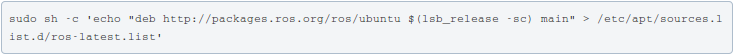
\includegraphics[width=1\textwidth]{Figures/Software/Install_ROS/Paso_1.png}
\end{center}

\subsection{Configura tus llaves}

%cita
\begin{center}
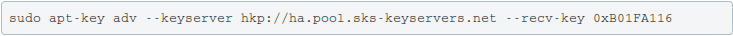
\includegraphics[width=1\textwidth]{Figures/Software/Install_ROS/Paso_2.png}
\end{center}

Puedes intentar el siguiente comando adhiriendo \textbf{:80} si tienes el error \textbf{gpg: keyserver timed}

%cita
\begin{center}
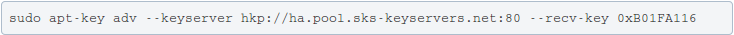
\includegraphics[width=1\textwidth]{Figures/Software/Install_ROS/Paso_3.png}
\end{center}

\subsection{Instalación}
Primero asegúrate que el índice de tu paquete ``Debian'' este actualizado

%cita
\begin{center}
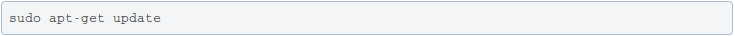
\includegraphics[width=1\textwidth]{Figures/Software/Install_ROS/Paso_4.png}
\end{center}

Si estás usando Ubuntu Trusty 14.04.2 y experimentas problemas de dependencia durante la instalación de ROS, debes 
instalar algunas dependencias del sistema adicionales.

%cita
\begin{center}
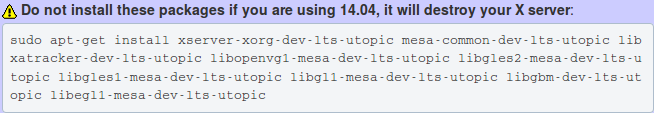
\includegraphics[width=1\textwidth]{Figures/Software/Install_ROS/Paso_5.png}
\end{center}

(Do not install the above package if you are using 14.04, it will destroy your X server)\\
Alternativamente, intenta instalando esto para arreglar problemas de\\ dependencia: 

\begin{center}
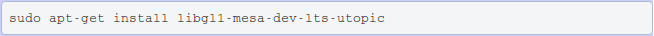
\includegraphics[width=1\textwidth]{Figures/Software/Install_ROS/Paso_6.png}
\end{center}

Hay muchas diferentes bibliotecas y herramientas en ROS. proveen 4 diferentes configuraciones para que inicies. Puedes 
también instalar los paquetes de ROS individualmente.\\

\textbf{Desktop-Full Install: (Recomendado)}: ROS, rqt, rviz, bibliotecas generales de robot, simuladores 2D/3D y 
percepción 2D/3D\\


\begin{center}
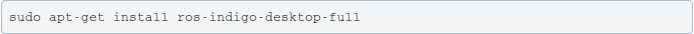
\includegraphics[width=1\textwidth]{Figures/Software/Install_ROS/Paso_7.png}
\end{center}

\textbf{Desktop install:}ROS, rqt, rviz, y bibliotecas de robots en general

\begin{center}
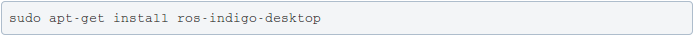
\includegraphics[width=1\textwidth]{Figures/Software/Install_ROS/Paso_8.png}
\end{center}

\textbf{ROS-Base: (Bare Bones) Paquetes de ROS, construcción y bibliotecas de comunicación. Sin herramientas GUI}

\begin{center}
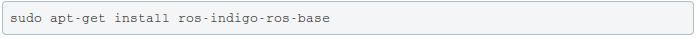
\includegraphics[width=1\textwidth]{Figures/Software/Install_ROS/Paso_9.png}
\end{center}

\textbf{Paquete individual:} Puedes además instalar un paquete especifico de ROS (remplaza)

\begin{center}
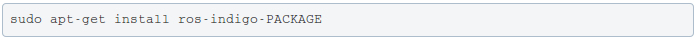
\includegraphics[width=1\textwidth]{Figures/Software/Install_ROS/Paso_10.png}
\end{center}

e.g.

\begin{center}
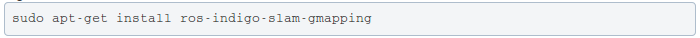
\includegraphics[width=1\textwidth]{Figures/Software/Install_ROS/Paso_11.png}
\end{center}

Para encontrar paquetes disponibles, utiliza:

\begin{center}
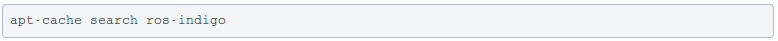
\includegraphics[width=1\textwidth]{Figures/Software/Install_ROS/Paso_12.png}
\end{center}

\subsection{Inicializar rosdep}
Antes de que puedas usar ROS, necesitaras inicializar rosdep. Rosdep le permite instalar fácilmente las dependencias 
del sistema para la fuente que buscas compilar y requiere correr algunos componentes del núcleo (Core) en ROS.

\begin{center}
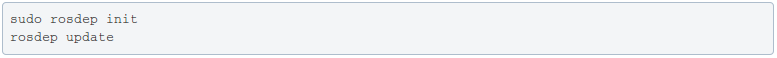
\includegraphics[width=1\textwidth]{Figures/Software/Install_ROS/Paso_13.png}
\end{center}

\subsection{Configuración del entorno}

Es conveniente si las variables del entorno de ROS son añadidas automáticamente a tu bash session cada vez que un 
nuevo shell es ejecutado. 

\begin{center}
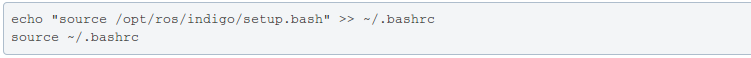
\includegraphics[width=1\textwidth]{Figures/Software/Install_ROS/Paso_14.png}
\end{center}

Si tienes mas de una distribución de ROS instalada; ~/.bashrc sólo debe generarse la configuración. bash para 
la version que utilizas actualmente.\\

Si sólo buscas cambiar el entrono de tu shell actual, puedes escribir:

\begin{center}
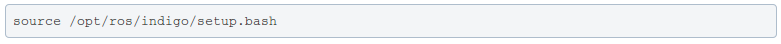
\includegraphics[width=1\textwidth]{Figures/Software/Install_ROS/Paso_15.png}
\end{center}

Si usas zhs en lugar de bash necesitas correr los siguientes comandos para configurar tu shell:

\begin{center}
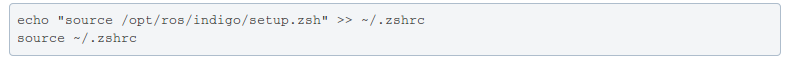
\includegraphics[width=1\textwidth]{Figures/Software/Install_ROS/Paso_16.png}
\end{center}

\subsection{rosinstall}

Rosinstalla es una linea de comando frecuentemente usada en ROS que es distribuida separadamente. te permite 
descargar fácilmente muchos arboles de fuente para los paquetes de ROS con un comando.

\begin{center}

\includegraphics[width=1\textwidth]{Figures/Software/Install_ROS/Paso_17.png}
\end{center}

\section{Instalación de PrimeSense drivers}

\begin{Verbatim}[fontsize=\footnotesize]
  sudo apt-get install freeglut3-dev pkg-config build-essential libxmu-dev libxi-dev
  libusb-1.0-0-dev doxygen graphviz mono-complete
\end{Verbatim}
\section{Instalación de OpenCV 2.4.9}

\begin{Verbatim}[fontsize=\footnotesize]
  sudo apt get update
  sudo apt-get install build-essential libgtk2.0-dev libjpeg-dev libtiff4-dev
      libjasper-dev libopenexr-dev cmake python-dev python-numpy python-tk
      libtbb-dev libeigen3-dev yasm libfaac-dev libopencore-amrnb-dev
      libopencore-amrwb-dev libtheora-dev libvorbis-dev libxvidcore-dev
      libx264-dev libqt4-dev libqt4-opengl-dev sphinx-common texlive-latex-extra
      libv4l-dev libdc1394-22-dev libavcodec-dev libavformat-dev libswscale-dev
      default-jdk ant libvtk5-qt4-dev
cd ~
wget http://sourceforge.net/projects/opencvlibrary/files/opencv-unix/2.4.9/opencv-2.4.9.zip
unzip opencv-2.4.9.zip
cd opencv-2.4.9
mkdir build
cd build
cmake -D WITH_TBB=ON -D BUILD_NEW_PYTHON_SUPPORT=ON -D WITH_V4L=ON -D INSTALL_C_EXAMPLES=ON
      -D INSTALL_PYTHON_EXAMPLES=ON -D BUILD_EXAMPLES=ON -D WITH_QT=ON -D WITH_OPENGL=ON
      -D WITH_VTK=ON -D WITH_OPENNI=ON -D WITH_OPENCL=OFF ..
make
sudo make install
sudo echo "/usr/local/lib" >> /etc/ld.so.conf.d/opencv.conf
sudo ldconfig
\end{Verbatim}

\section{Instalando otros paquetes de ROS}
\begin{verbatim}
    sudo apt-get install ros-indigo-amcl
    sudo apt-get install ros-indigo-tf2-bullet
    sudo apt-get install ros-indigo-fake-localization
    sudo apt-get install ros-indigo-map-server
    sudo apt-get install ros-indigo-sound-play
    sudo apt-get install ros-indigo-pocketsphinx
\end{verbatim}

\end{document}
